\section{Results}
\label{sec:results}

We test the four proposed dispatching strategies in the Zurich scenario with ten
runs per fleet size and strategy.% Commented out to reduce works / sh
%Since the dispatchers rely on free flow speeds in the network
%for their routing when the simulation starts, we let each run perform 20 iterations
%in which the dispatcher step by step senses the traffic conditions, e.g. how to
%avoid traffic jams at peak hours.
The dispatching stages of all algorithms are called once every 60 seconds in
simulated time, while the rebalancing periods for the feedforward and feedback
dispatcher are five minutes and 20 minutes, respectively. Those values have been
obtained from prior simulation runs.

For Zurich, the times with peak congestion and, hence, longest travel times
are from 6:30pm to 9:00am and from 4:30pm to 6:30pm. Figure \ref{fig:mean_peak_waiting_times}
shows the average customer wait time over the whole day and just for peak hours.
While the simple heuristic approach consistently yields the longest wait times
for any fleet size, the feedback dispatcher performs best. The bipartite matching
performs in between, since it is based on an optimal request assignment, but does
not do any rebalancing. Since both algorithms rely on rebalancing, the two linear
programs have very similar performance. The feedback algorithm seems to have a
slight advantage, especially for average wait time over the whole day, because it
is able to react to actuallly observed demand more precisely.

Assuming that 5 minutes at peak times are an acceptable wait time, that value is
achieved with a fleet of 10,000 vehicles for the heuristic, but with only 8,700
for the feedback dispatcher.

\captionsetup[subfigure]{width=0.9\textwidth}

\begin{figure}
    \centering
    \begin{subfigure}[t]{0.495\textwidth}
        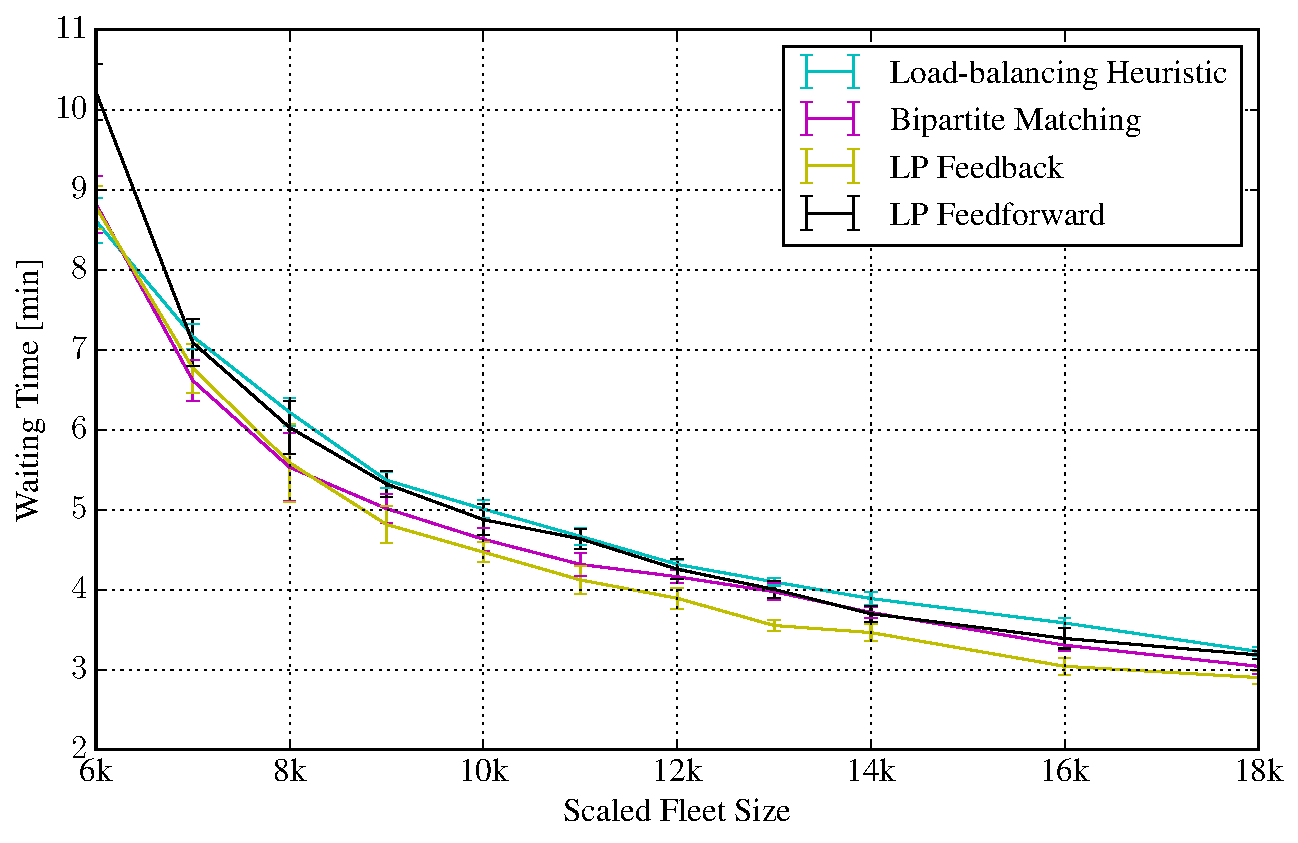
\includegraphics[width=1.0\textwidth]{figures/mean_peak_waiting_times.pdf}
        \caption{Average waiting time for an AV to arrive at peak times (solid) and over the entire day (dashed)}
        \label{fig:mean_peak_waiting_times}
    \end{subfigure}\hfill
    \begin{subfigure}[t]{0.495\textwidth}
        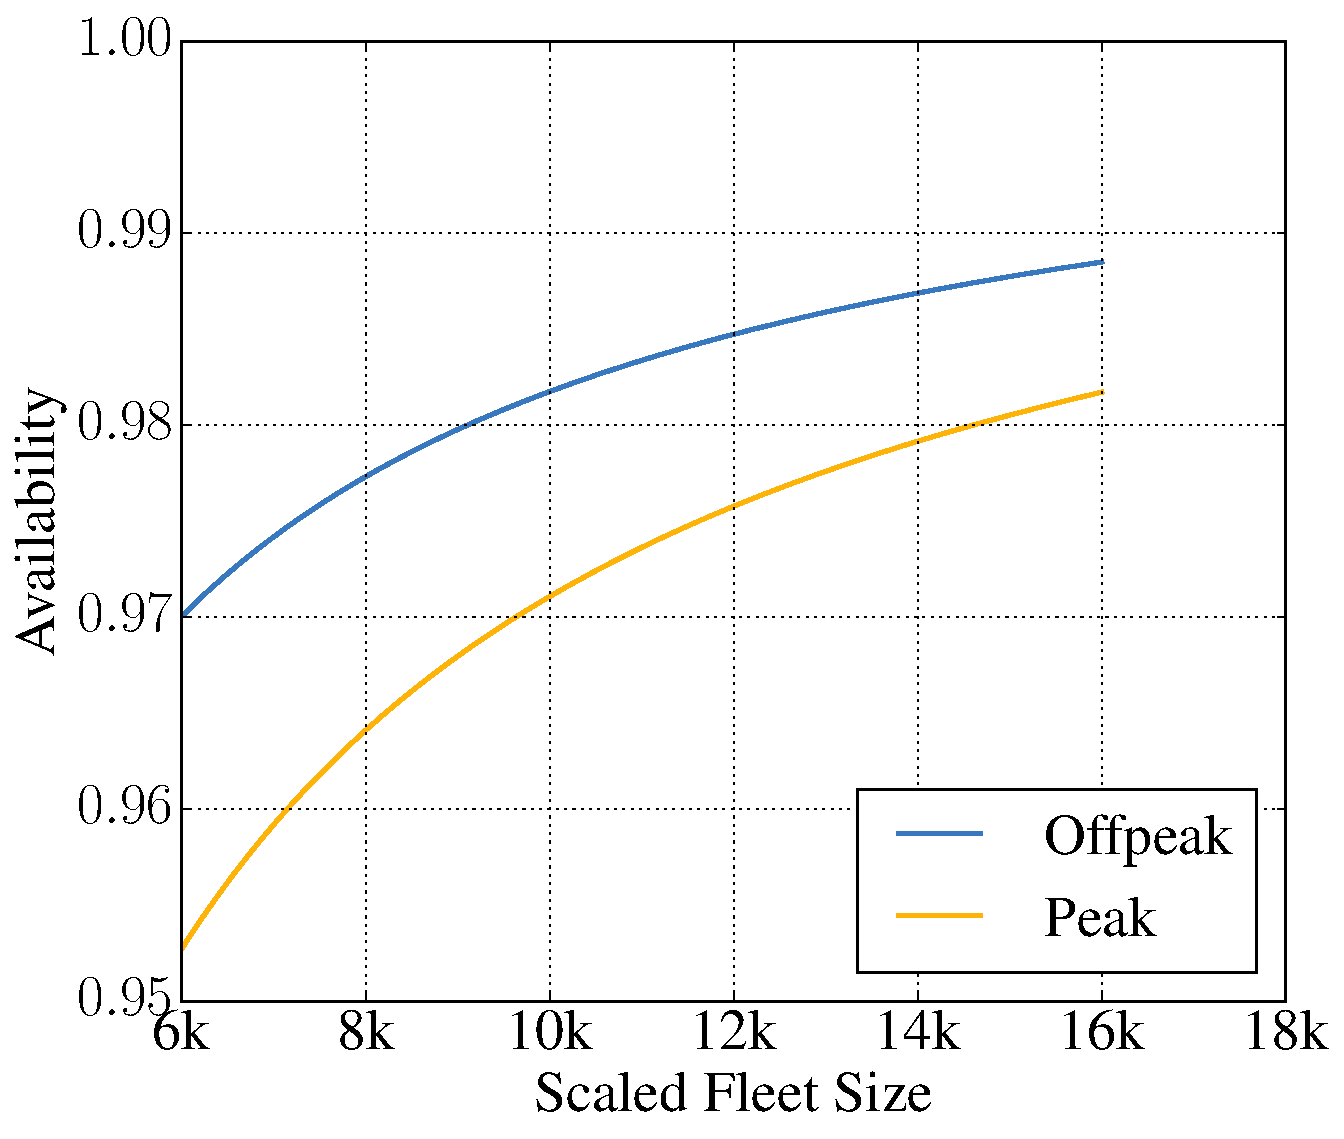
\includegraphics[width=1.0\textwidth]{figures/availability.pdf}
        \caption{Probability of at least one AV being available whenever a request comes in
        [TODO: Passt das scaling so? /sh]}
        \label{fig:performanceavailability}
    \end{subfigure}
    \caption{Fleet performance metrics for different fleet sizes}
\end{figure}

%\begin{figure}
%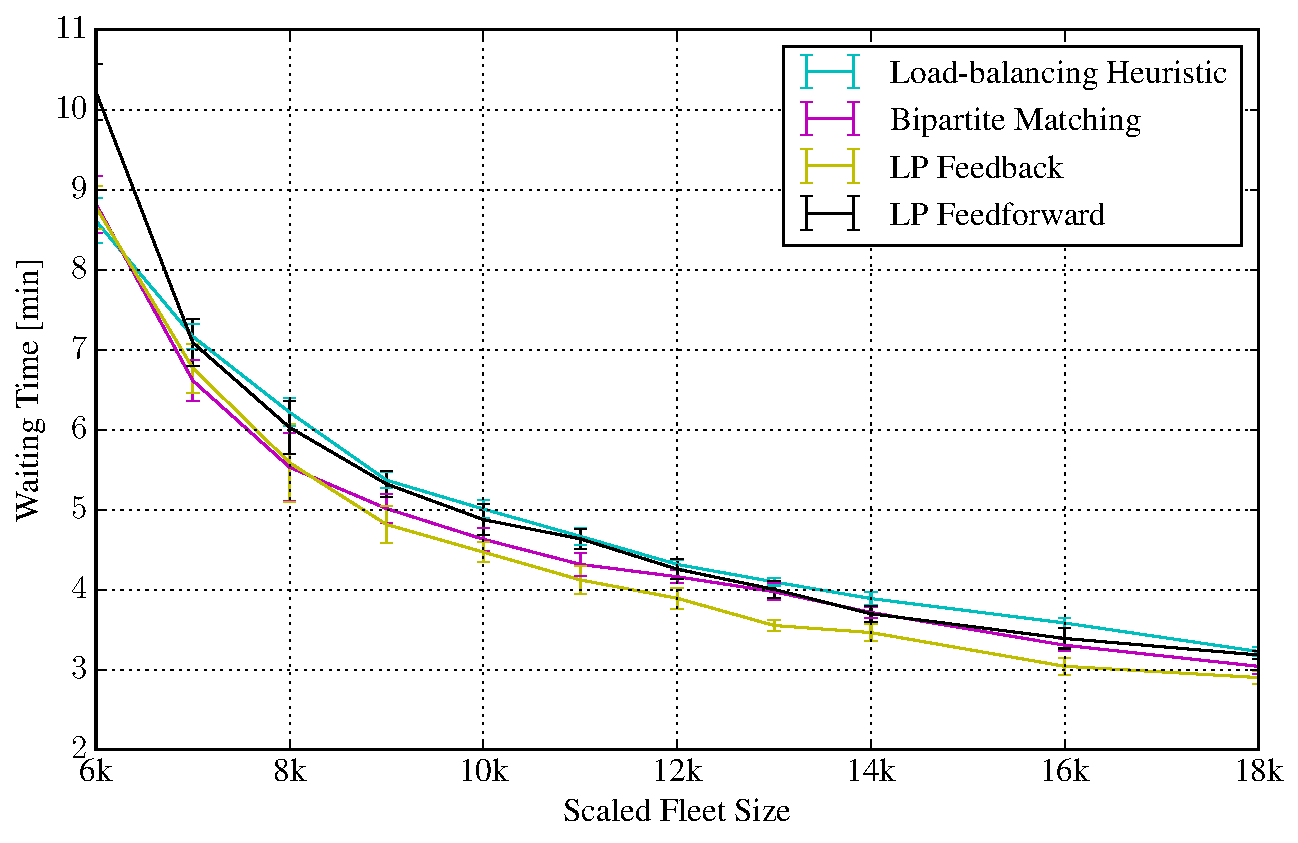
\includegraphics[width=1.0\textwidth]{figures/mean_peak_waiting_times.pdf}
%\caption{Average waiting time for an AV to arrive at peak times (solid) and over the entire day (dashed)}
%\label{fig:mean_peak_waiting_times}
%\end{figure}

Figure \ref{fig:distances} shows the distances that different service configurations
produce. On the left side the customer distance is shown, which stays constant
over all runs, while one can see that the pickup distance (middle, light) is decreasing
with larger fleet sizes and thus higher availability of vehicles. For the dispatchers
with rebalancing once can see that they add a surplus of mileage for rebalancing (right, dark)
such that the overall driven distance is rather stabilized over different fleet sizes.
This added mileage is used to provide the shorter travel times as presented above.
One can see that with similar wait times the feedback dispatcher operates more economically
by saving mileage compared to the feedforward algorithm.

\begin{figure}
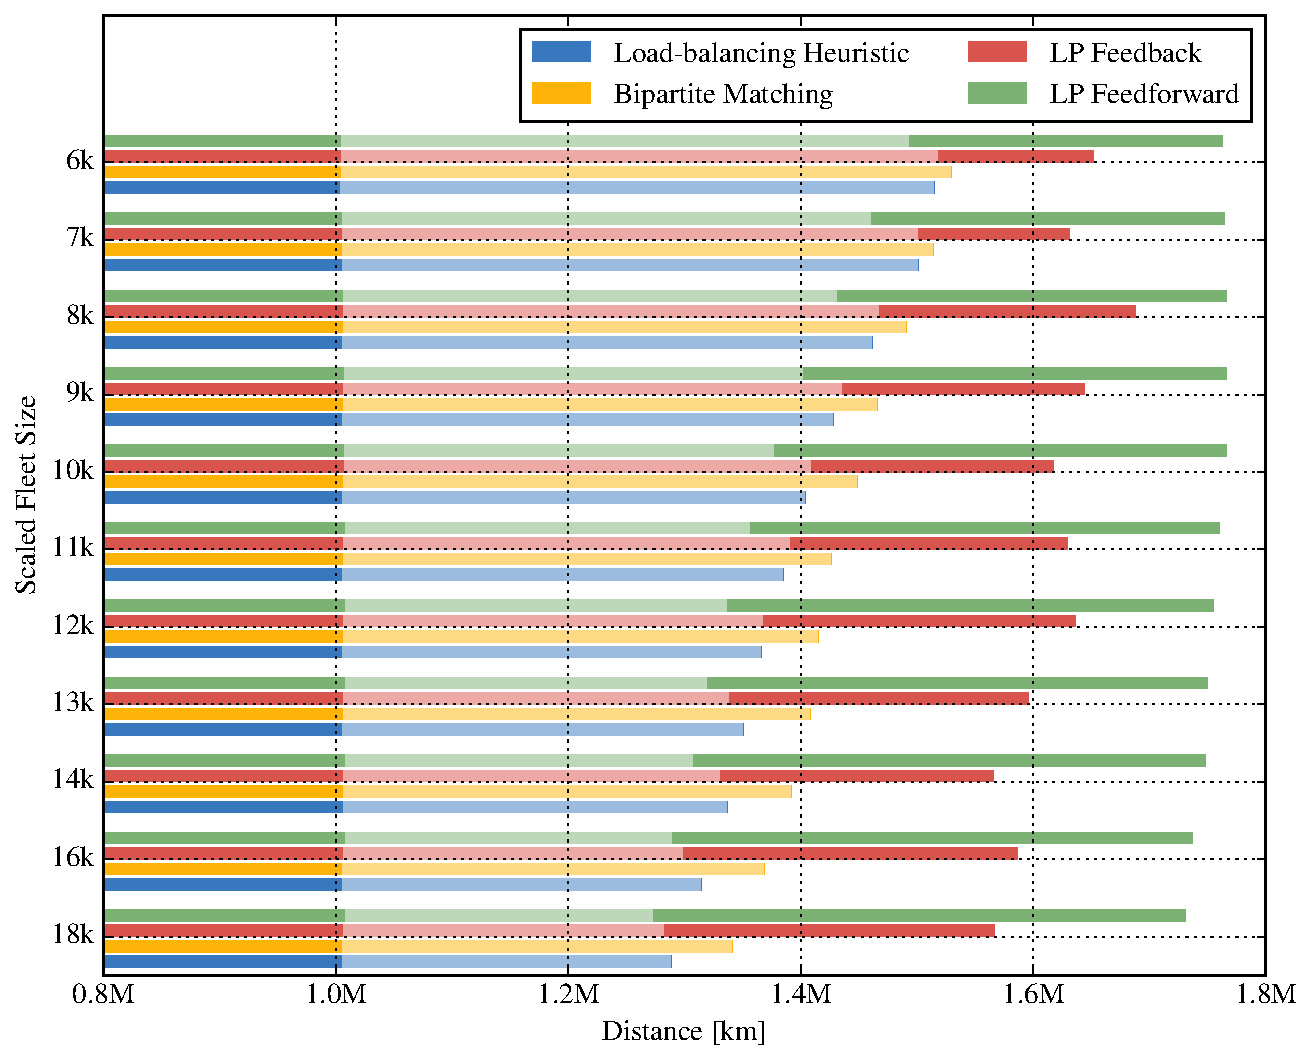
\includegraphics[width=1.0\textwidth]{figures/distances.pdf}
\caption{Driven accumulated distances for different fleet sizes. From left to right:
Customer distance (dark), empty pickup distance (light), empty rebalancing distance (light).}
\label{fig:distances}
\end{figure}

Finally, the occupancy of the fleet is measured. For a fleet size of 6,000
vehicles, they are busy serving a passenger for around 4.8h per day, while
this value drops to 2.16h for the maximum fleet size of 180,000. In both cases,
those numbers exceed the average 1.92h [TODO: Do we have an exact value for Switzerland? /sh] of today's vehicle fleet.

\subsection{Financial Analysis}
\label{sec:cost_analysis}

[TODO: REWORK FINANCIAL ANALYSIS AND ABSTRACT!!! -> Felix]



Based on the cost calculator for fleets of automated vehicles by Bösch et al. \cite{Bosch2016a}
 the costs of operating the AV services are computed from a number of key figures
 such as the occupancy, share of empty rides, among others. In Figure~\ref{fig:passenger_price}
 the resulting price is shown that the operators needs to ask his customers per
 kilometer if a profit margin of at least 3\% is targeted. Unsurprisingly, the value
  increases with larger fleet sizes, but a clear difference
between the algorithms can be observed. The simple heuristic is the most
costly operating scheme, while the feedback dispatcher can be operated with the
lowest passenger prices.


\captionsetup[subfigure]{width=0.9\textwidth}

\begin{figure}
    \centering
    \begin{subfigure}[t]{0.495\textwidth}
        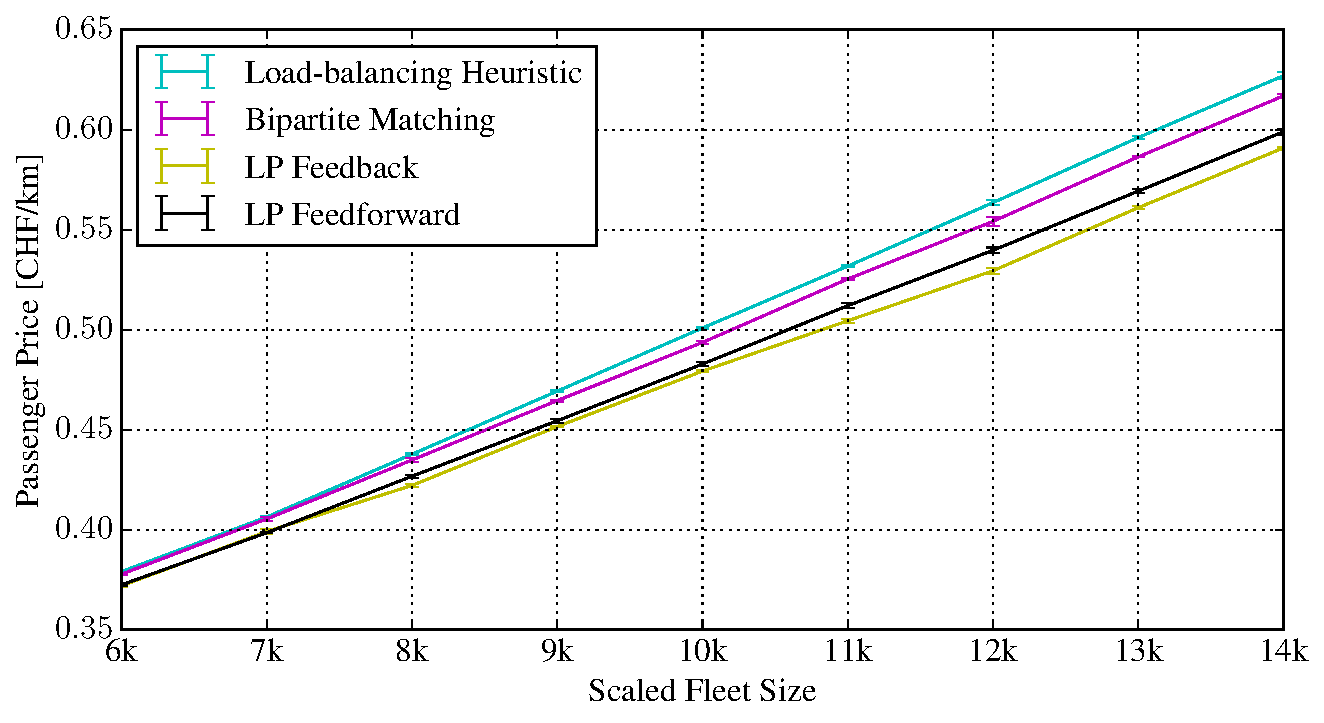
\includegraphics[width=1.0\textwidth]{figures/01_passenger_price.pdf}
        \caption{Minimum customer prices that an AV operator needs to charge with a profit margin of at least 3\%}
        \label{fig:passenger_price}
    \end{subfigure}\hfill
    \begin{subfigure}[t]{0.495\textwidth}
        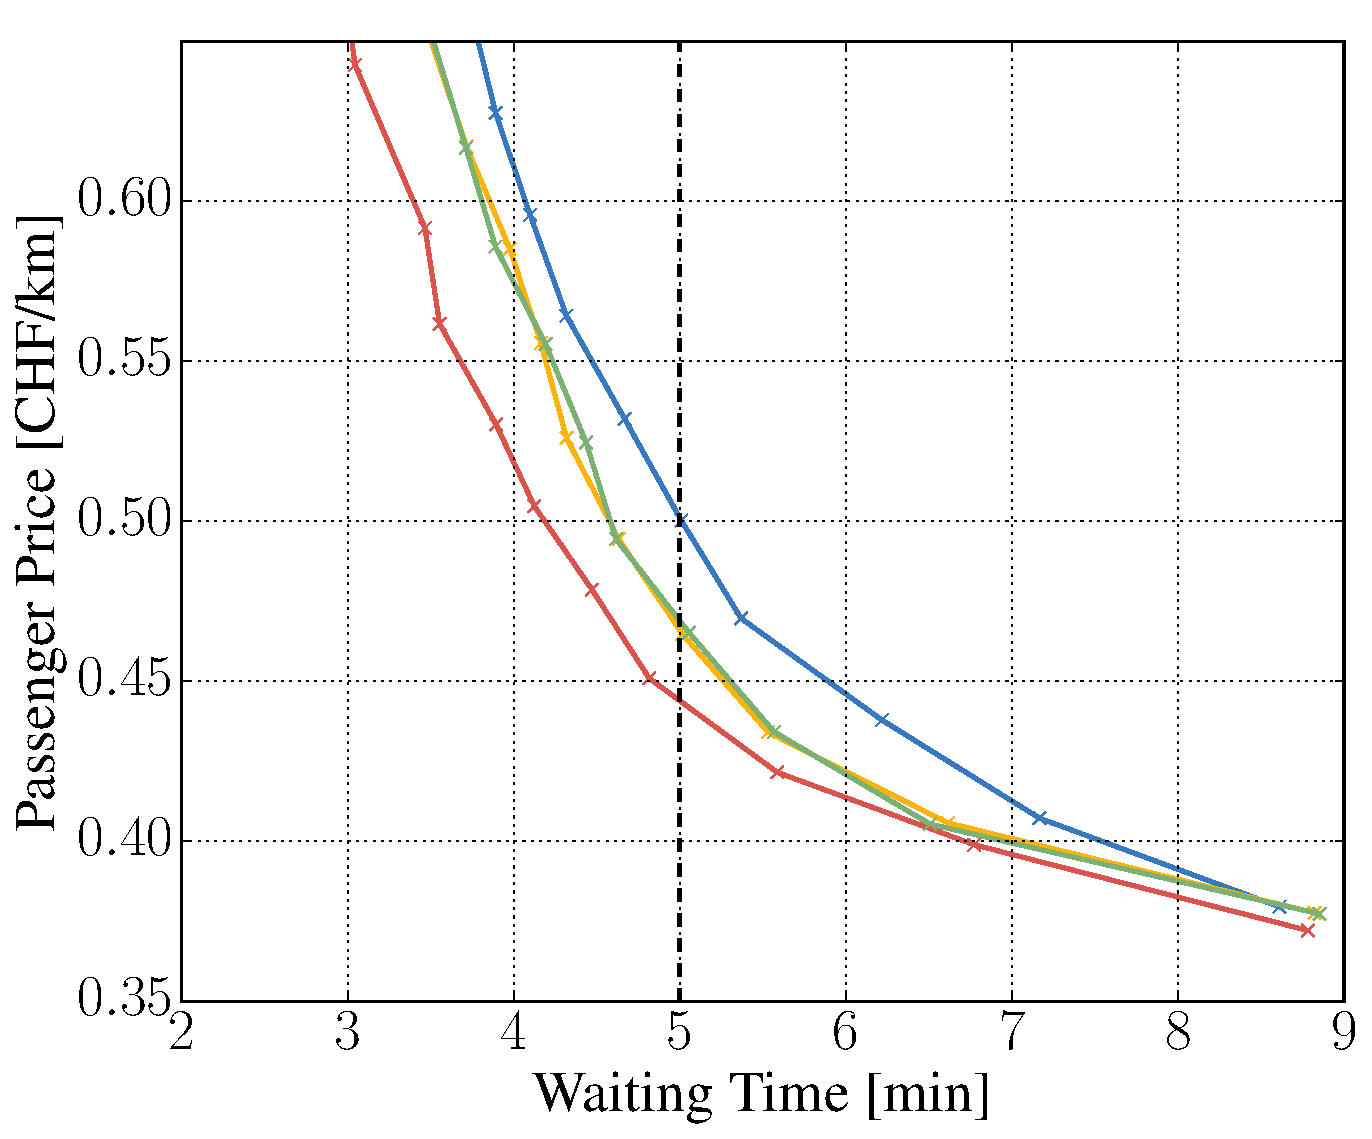
\includegraphics[width=1.0\textwidth]{figures/time_vs_price.pdf}
        \caption{Comparison plot of offered wait times and minimum service prices for the
        simulated fleet configurations}
        \label{fig:time_vs_price}
    \end{subfigure}
    \caption{Analysis of fleet configurations from the customer perspective}
\end{figure}

Compared to the price of a taxi operator in Zurich (base price 8 CHF plus 5 CHF/km, \cite{StadtZurich2014})
the computed prices are extremely low. Hence, an automated service would clearly
push conventional taxi operators out of the market. The variable costs of a today's private vehicle (0.26 CHF/km, \cite{TCS2016}) are lower than the calculated prices for the AV-services, independent of the algorithm. Considering the full costs of a private vehicle which amount to 0.7 CHF/km \cite{TCS2016} however, it can be concluded that AV-services are only more expensive for large fleet sizes. Nonetheless, compared to
(subsidized) prices for mass transit (0.25 CHF/passenger kilometer, \cite{Bosch2016a}), the services are more
expensive.

Therefore, the proposed AV services are highly attractive to car users, but may
not be able to compete with subsidized mass transit. On the other hand, AVs
allow for more direct trips and thus for savings in travel time. Further studies
may analyse how these affect the attractiveness of the AMoD services.

The expected wait time and the price of the service are the two decisive factors
for customers deciding to use one or another operator, therefore it is important
to compare these variables for different control methods. Figure \ref{fig:time_vs_price}
shows the price that a specific operator configuration (fleet size and dispatcher)
needs to charge to be profitable in comparison to the wait time that this operator is offering.
At a wait time of five minutes an operator would be able to offer a satisfactory service for
around 0.45 CHF with the feedback dispatcher, while he would need to charge 0.50 CHF
with the simple load-balancing heuristic.

%The better the level of service of the operator is, the larger this margin becomes.
